\subsection{End-to-end mobility using \auspice}
\label{sec:case}

Next, we evaluate whether \auspice\ can serve as the basis of a complete end-to-end mobility solution (refer Fig.\ref{fig:4mobility}). To this end, we have developed \msocket, a user-level socket library that interoperates with \auspice. \msocket\ has support for all four types of endpoint mobility. Using \auspice, \msocket\  supports connection migration, multipath communication, and mobile-to-mobile communication despite address-translating middleboxes using a distributed proxy service. A detailed description of \msocket's design and implementation is the subject of a separate 20-page anonymized techreport \cite{msocketTR}. Here, we {\em use} \msocket\ to demonstrate \auspice's strengths.

\subsubsection{Simultaneous endpoint mobility}

\begin{figure}[htbp]
\begin{center}
\vspace{-1in}
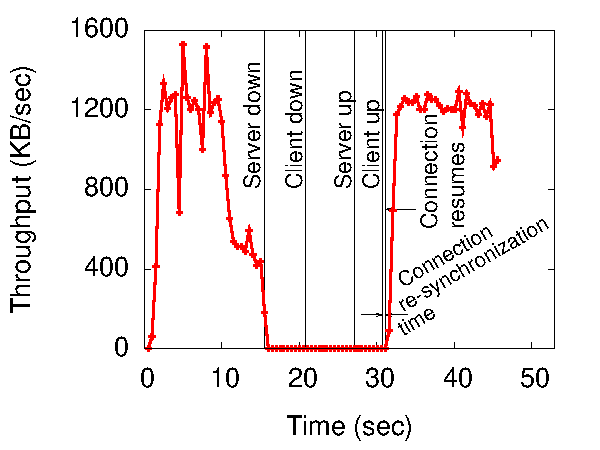
\includegraphics[scale=0.3]{auspice/figure/SimulMig}
\vspace{-1in}
\caption{Simultaneous endpoint mobility in $\approx$ 2 RTTs}
\vspace{-0.2in}
\label{fig:SimulMig}
\end{center}
\end{figure}

Figure \ref{fig:SimulMig} shows an experiment involving simultaneous mobility. The client is an Android phone using \msocket\ via a WiFi interface to connect to a publicly addressable Planetlab machine at time 0. The server and client shut down their interfaces respectively around 15 and 20 sec. After this, the server restarts its interface and starts listening on a different port and updates \auspice\ with this information. After that, the client restarts its interface and attempts to re-synchronize the connection. This re-synchronization time is roughly 300ms as shown and consists of the following delays. The client performs a query to \auspice\ to resolve the server's GUID to its new socket address (IP, port), which takes roughly 50ms and mostly corresponds to the round-trip delay between the client and the \auspice\ nameserver. The remaining 250ms roughly correspond to 2 RTTs of delay between the client and the server that are separated by a round-trip delay of 120ms.

\subsubsection{Context-aware delivery}
\label{sec:context}

Next, we show a proof-of-concept of context-aware communication, a novel communication primitive enabled by \auspice's extensible key-value store API. \auspice\ allows developers to bind an \msocket\ not only to human-readable names or GUIDs, but also to abstract context descriptors like \verb+msocket.bind("[geoloc:+\\
\verb+[lat,long],radius]")+. Any writes to this \msocket\ will be reliably delivered to all GUIDs that belong to the geo-fence created by the context descriptor. Underneath the covers, \msocket\ issues a call to \auspice\ to create on-demand a ``group GUID" that is an  GUID with a membership field consisting of a set of member GUIDs, and this member set is returned to \msocket. \msocket\ internally resolves each member GUID to its socket address (IP, port) and establishes a regular \msocket\ connection to reliably deliver messages.



%\begin{figure*}[ht]
%\vspace{0.05in}
%\begin{minipage}[b]{0.3\linewidth}
%\centering
%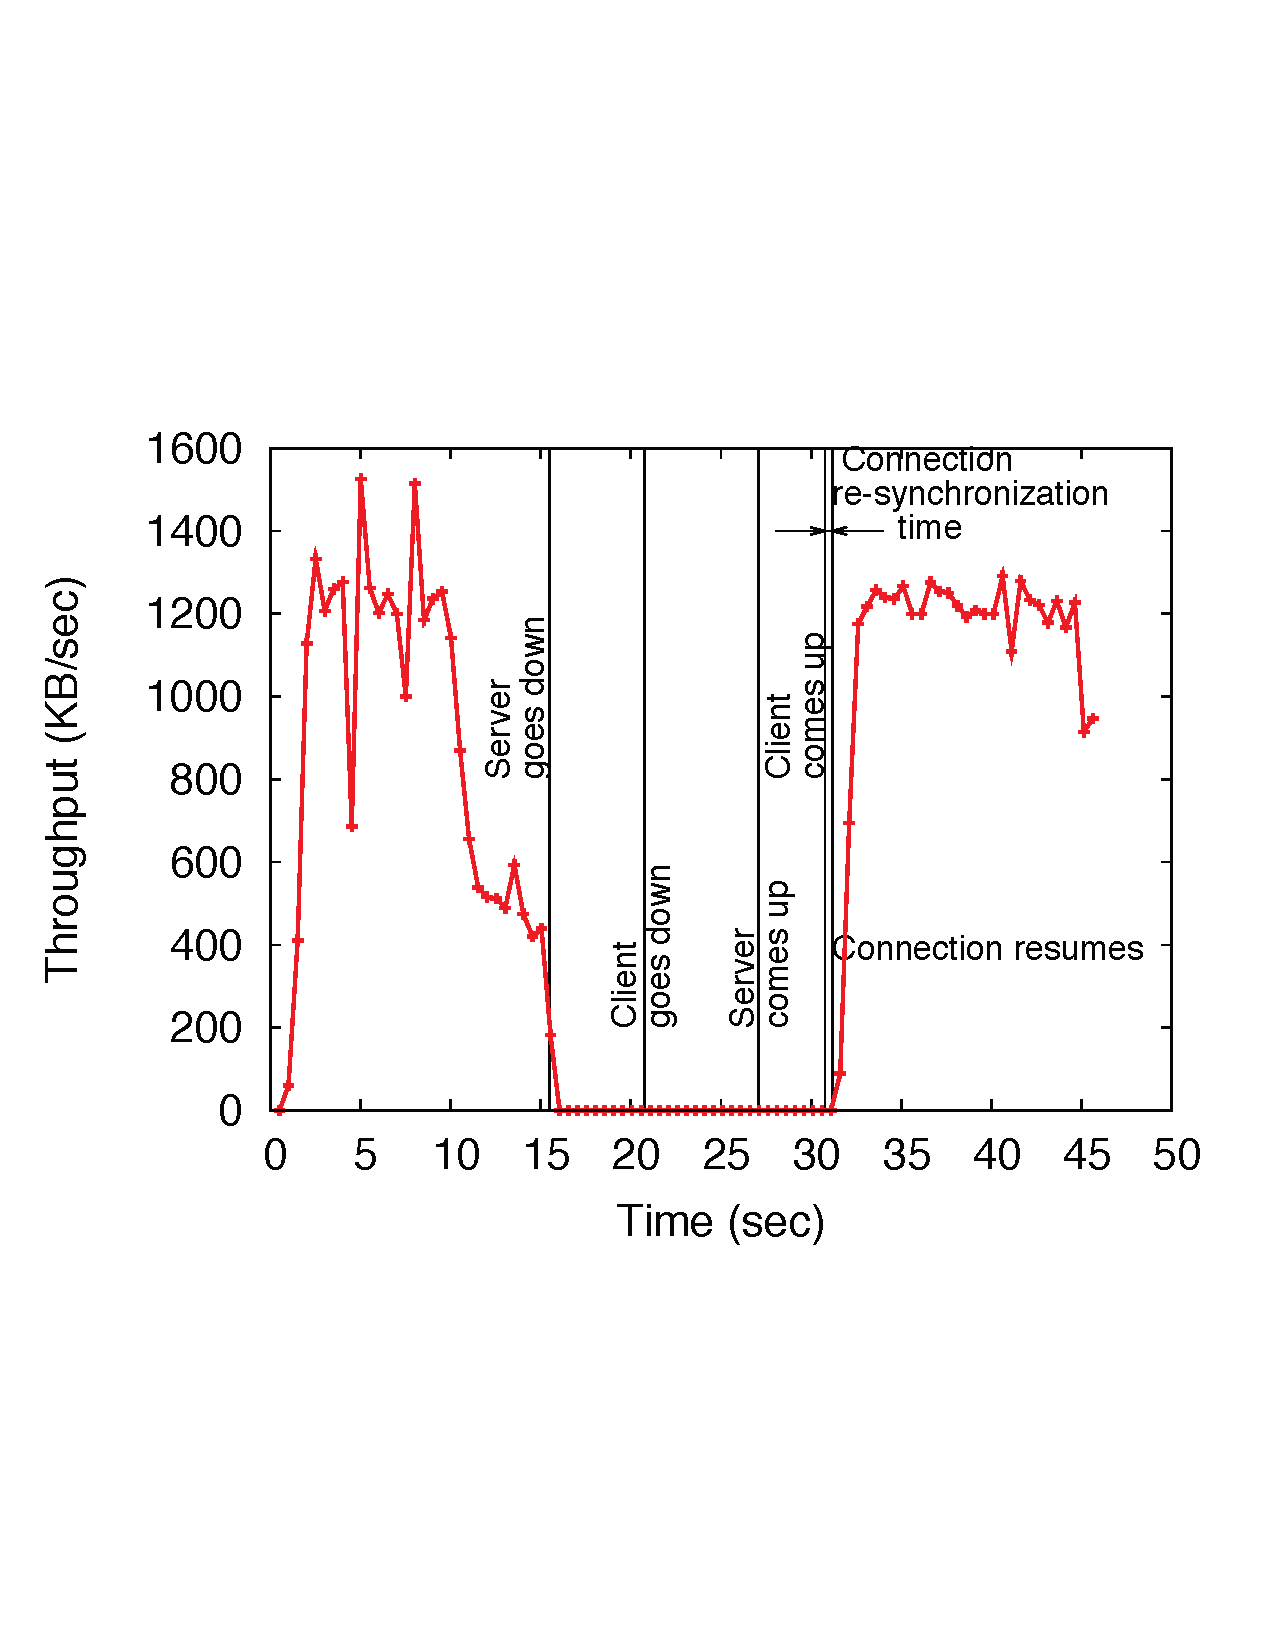
\includegraphics[scale=0.28]{figure/SimulMig}
%\caption{Simultaneous mobility}
%\end{minipage}
%\begin{minipage}[b]{0.7\linewidth}
%\centering
%{\includegraphics[scale=0.28]{figure/5MemberTimeline}
%\label{fig:5MemberTimeline}}
%{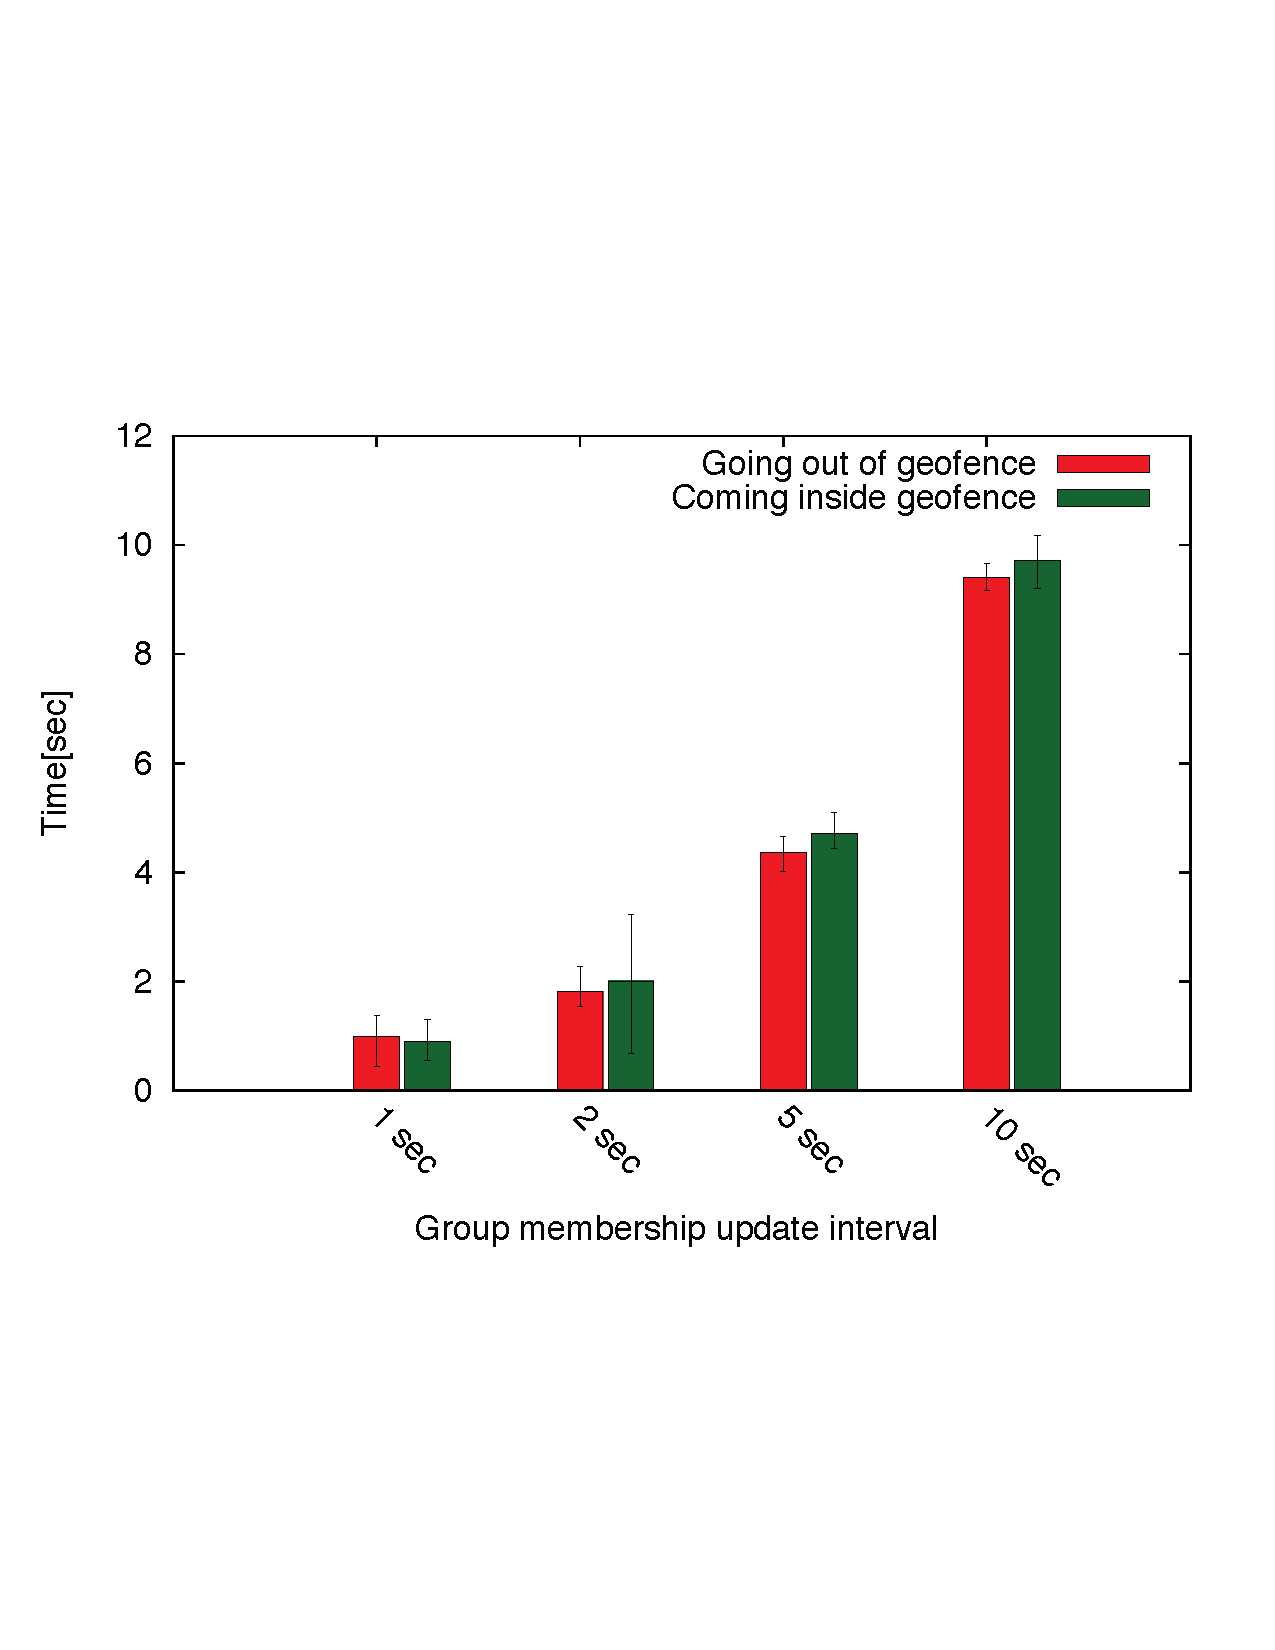
\includegraphics[scale=0.28]{figure/geoCastStaleness}
%\label{fig:geoCastStaleness}}
%\caption{Context-aware delivery}
%\end{minipage}
%%\vspace{-0.25in}
%\end{figure*}



\begin{figure}[t]
\begin{center}
\vspace{-0.8in}
{\includegraphics[scale=0.3]{auspice/figure/5MemberTimeline}
\label{fig:5MemberTimeline}
}
\vspace{-1.5in}
{
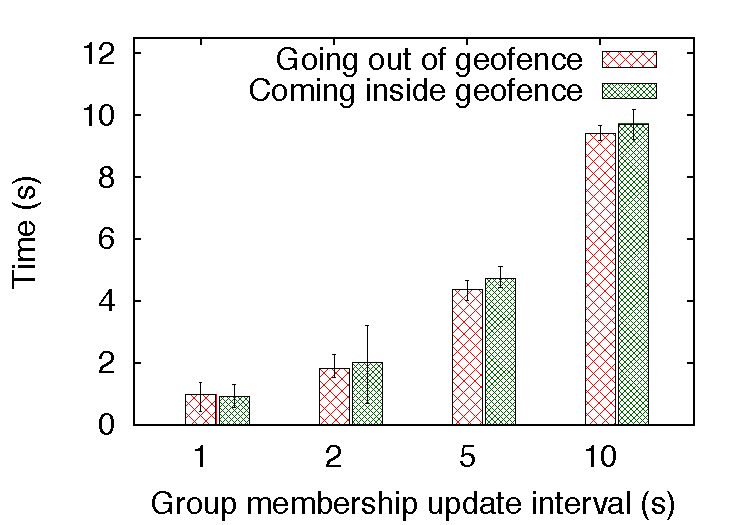
\includegraphics[scale=0.3]{auspice/figure/geoCastStaleness}
\label{fig:geoCastStaleness}
}
\vspace{-0.85in}
\caption{Context-aware delivery}
\vspace{-0.2in}
\end{center}
\end{figure}

%
%\begin{figure}[htbp]
%\begin{center}
%{\includegraphics[scale=0.3]{figure/5MemberTimeline}
%\label{fig:5MemberTimeline}
%}
%{
%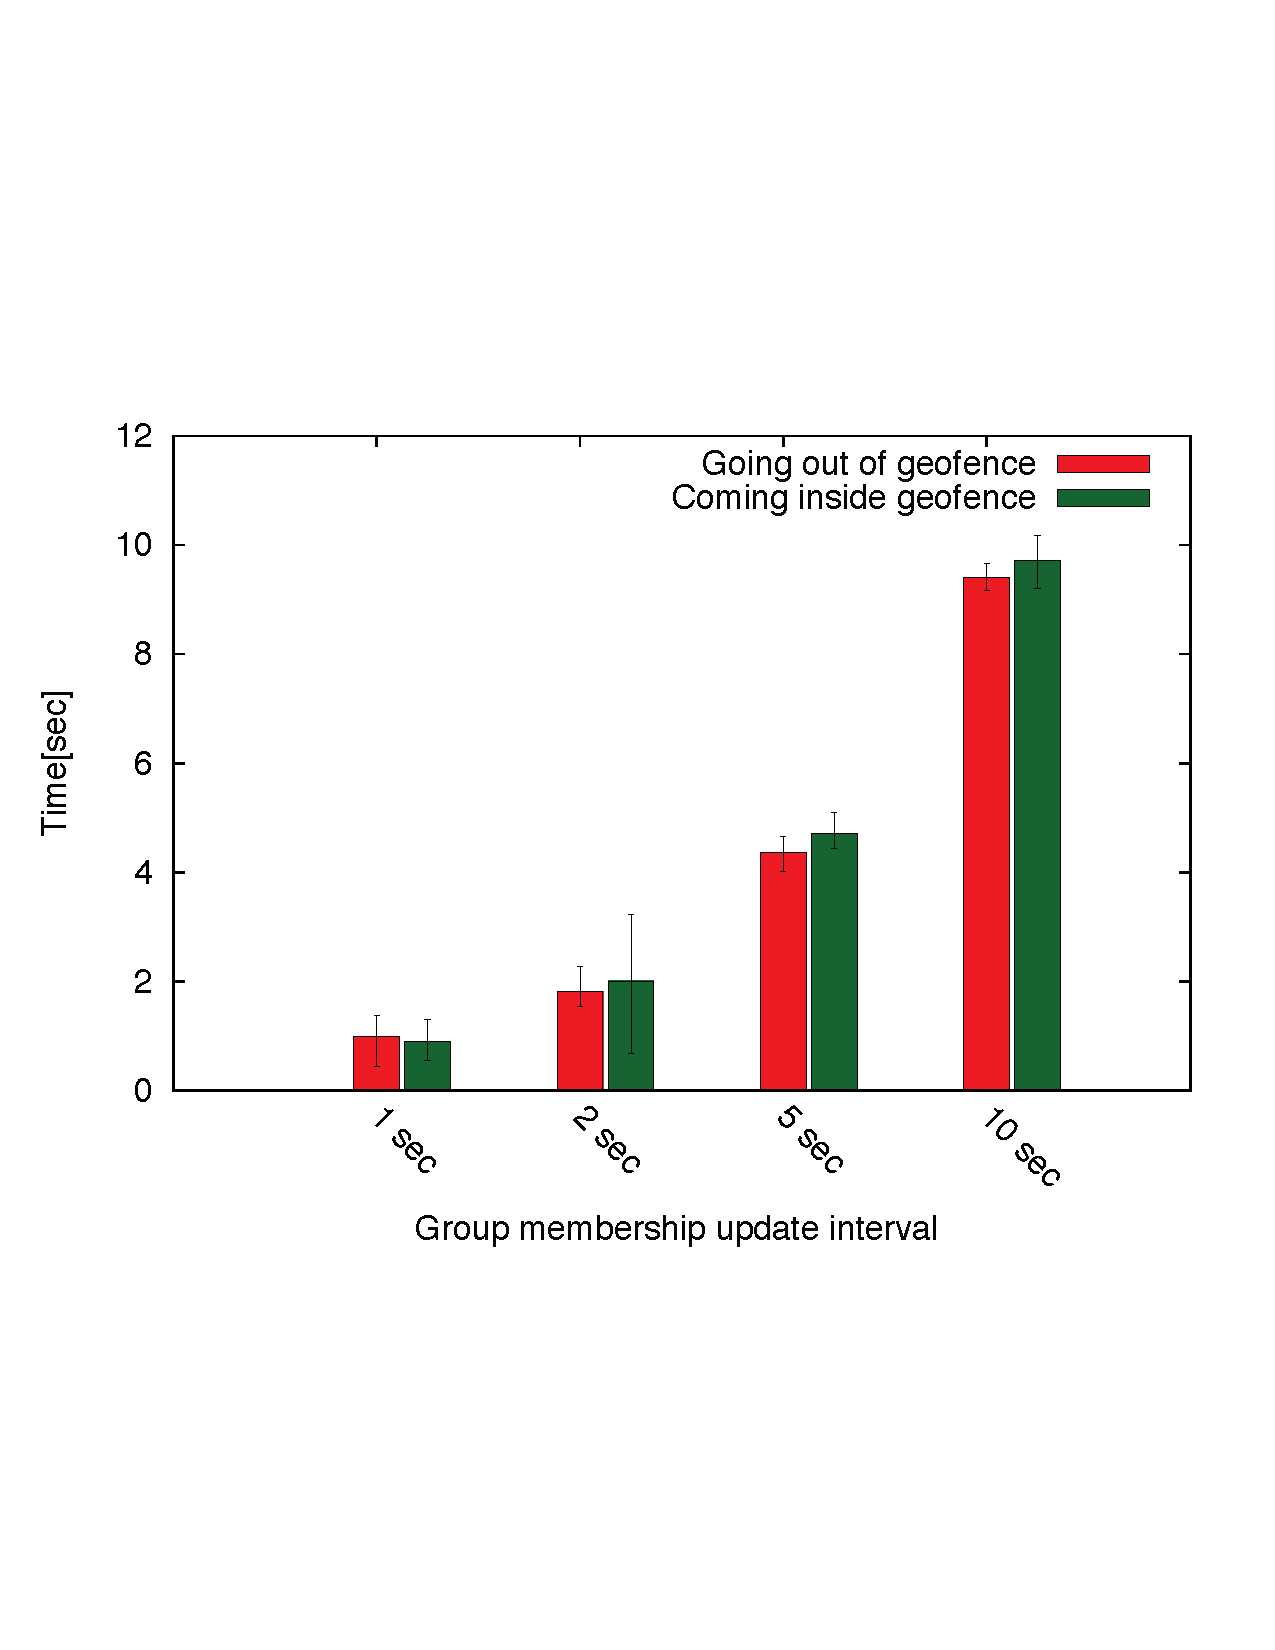
\includegraphics[scale=0.3]{figure/geoCastStaleness}
%\label{fig:geoCastStaleness}
%}
%\caption{Context-aware delivery}
%\end{center}
%\end{figure}

Fig. \ref{fig:5MemberTimeline} shows the results of an experiment involving a group creator (and message sender) on an Android phone and a number of potential members on Planetlab nodes, 5 of which fake-register their coordinates in \auspice\ so as to appear to be within the geo-fence created by the member. The RTT between the group creator and members is 125ms. The figure shows that group creation, a single call to \auspice\ that returns all member GUIDs, takes roughly 200ms. Subsequently, an internal \msocket\ connect to each member involves another \auspice\ lookup to resolve the GUID to a socket address and connect in parallel to all 5 members, which takes 250-280ms. After this, the creator sends 3 short messages back-to-back that each take roughly 1 RTT to be reliably delivered.

Context-aware group GUIDs in \auspice\ are active, i.e., \auspice\ keeps the membership set refreshed so that if an existing member leaves or a new member arrives into the context-space, the group GUID gets updated accordingly. However, the refresh interval limits how responsive the context-aware communication is to member churn. Figure \ref{fig:geoCastStaleness} shows that the time after which a new member (an old member) walking into (leaving) the context-space starts (stops) getting messages is roughly commensurate to the refresh interval. 

All of the experiments in this section are meant to show proof-of-concept of \auspice's strengths. The details of optimizing context-aware queries in \auspice, reducing membership staleness, the socket API etc. \cite{msocketTR} are outside the scope of this paper. 












